\label{B1DATASECTION}
%\begin{figure}
%\begin{center}
%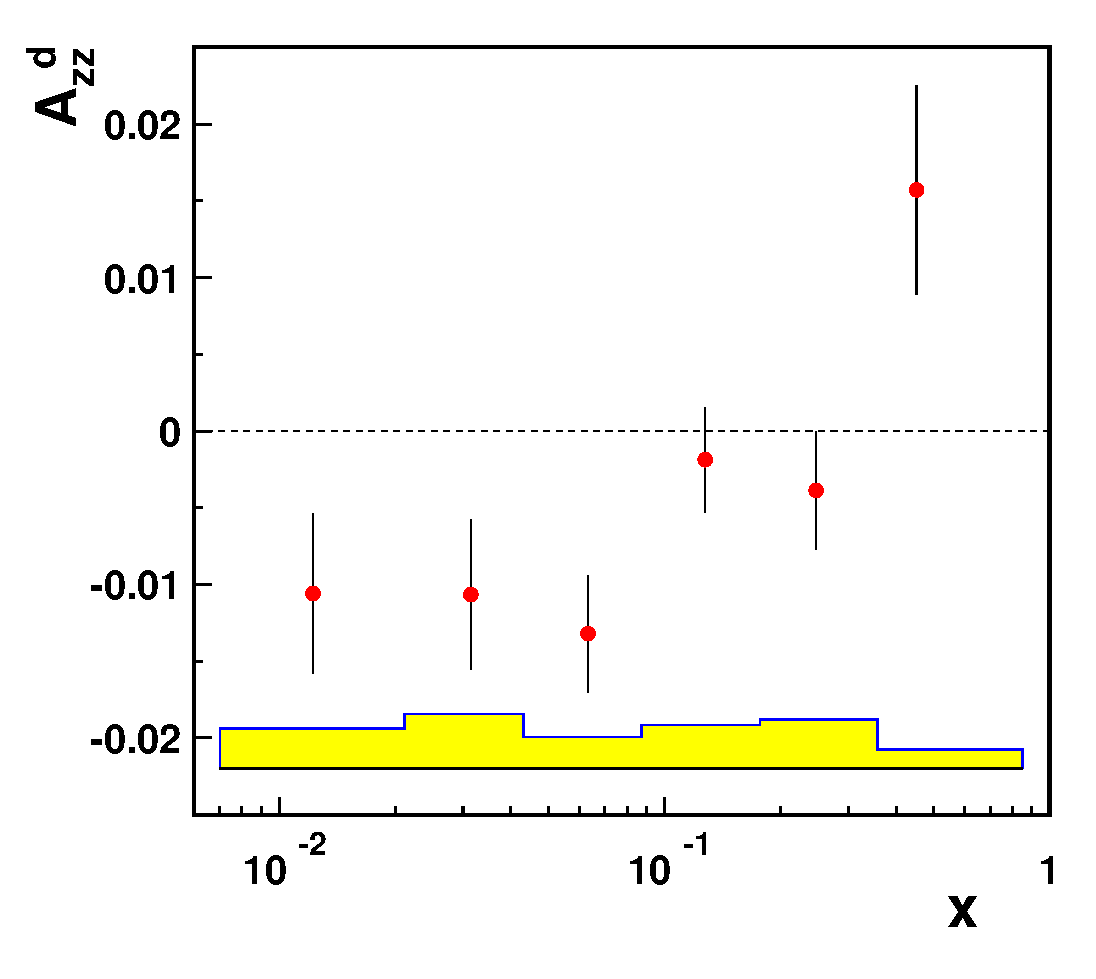
\includegraphics[angle=0,width=0.45\textwidth]{figs/azzfinal.eps}
%
%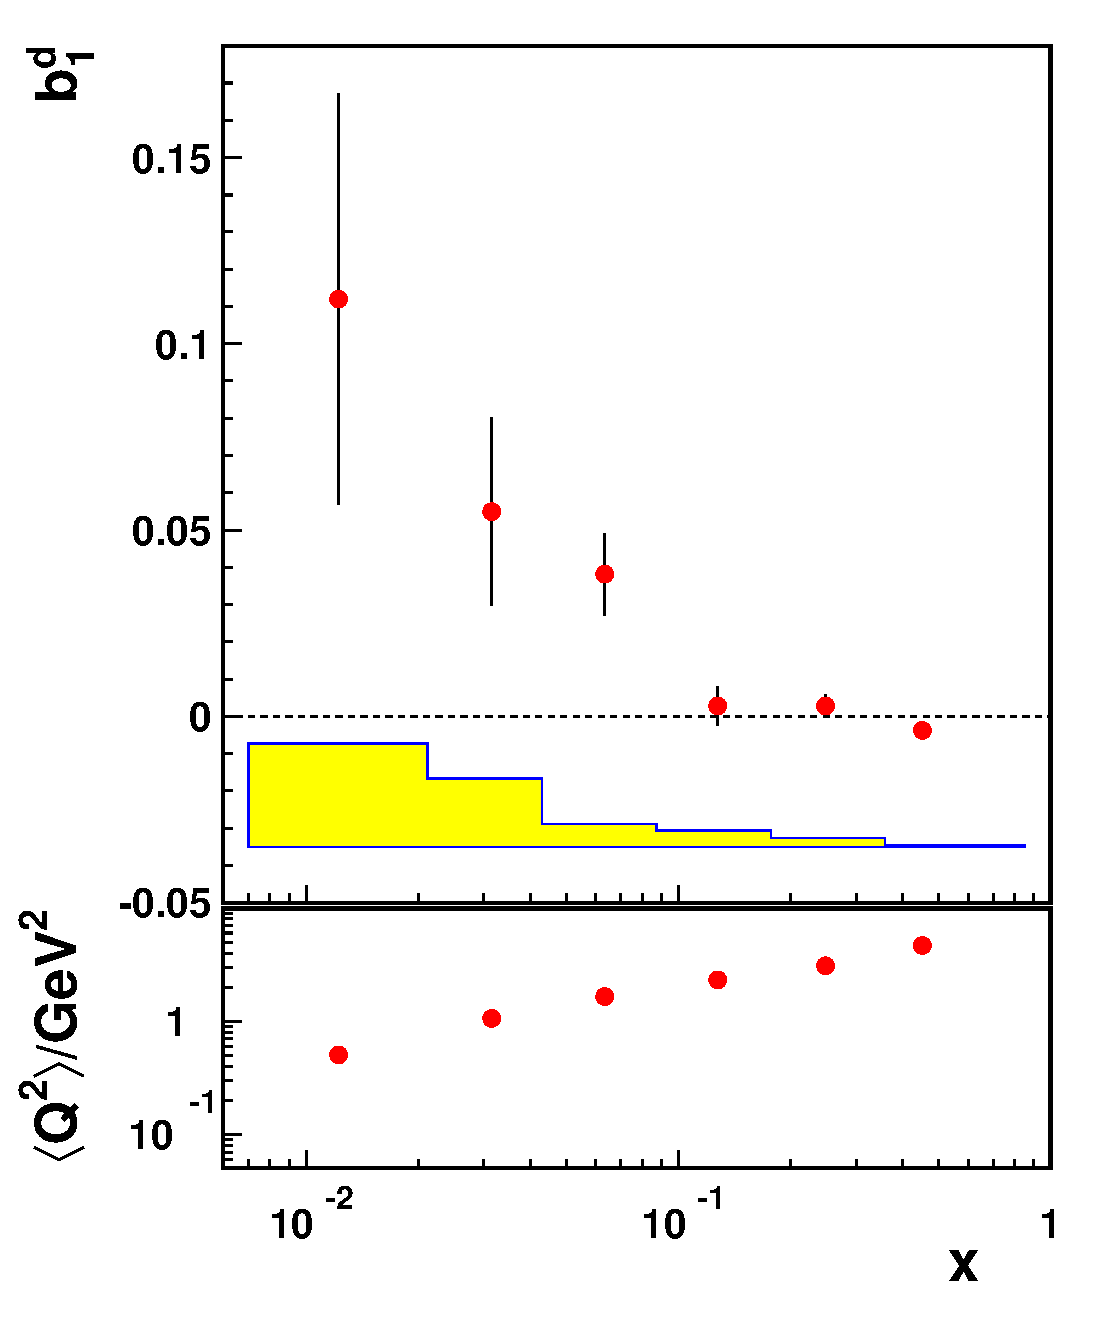
\includegraphics[angle=0,width=0.47\textwidth]{figs/b1final.eps}
%\caption{\label{HERMES_AZZ} {\bf Top:} HERMES measurement of the inclusive tensor asymmetry A$_{zz}$ of the deuteron.  
%{\bf Bottom:} HERMES measurement of the inclusive tensor structure function b$_1^d$ and the average $Q^2$ for each x-bin.  The error bands displays the total systematic uncertainty.
%{\it Reproduced from~\cite{Riedl:2005jq}.}}
%\end{center}\end{figure}

\begin{figure}
\begin{center}
\includegraphics[angle=0,width=0.45\textwidth]{figs/1.eps}
\hspace{0.5cm}
\includegraphics[angle=0,width=0.45\textwidth]{figs/2.eps}
\vspace{3cm}

\includegraphics[angle=0,width=0.45\textwidth]{figs/3.eps}
\caption{\label{HERMES_AZZ} {\bf Top}: HERMES~\cite{Riedl:2005jq} measurement of the inclusive tensor asymmetry A$_{zz}(x)$ and $xb_1(x)$ of the deuteron. {\bf Bottom} : The tensor structure function $b_1(x)$ without $x$-weighting, which reveals a steep rise as $x\to 0$. 
}
\end{center}\end{figure}

%\begin{figure}
%\begin{center}
%\includegraphics[angle=0,width=0.47\textwidth]{figs/2.eps}
%\caption{\label{HERMES_AZZ2} 
%HERMES~\cite{Riedl:2005jq} measurement of the inclusive tensor structure function b$_1^d$.  
%}
%\end{center}\end{figure}



%\begin{figure}
%\begin{center}
%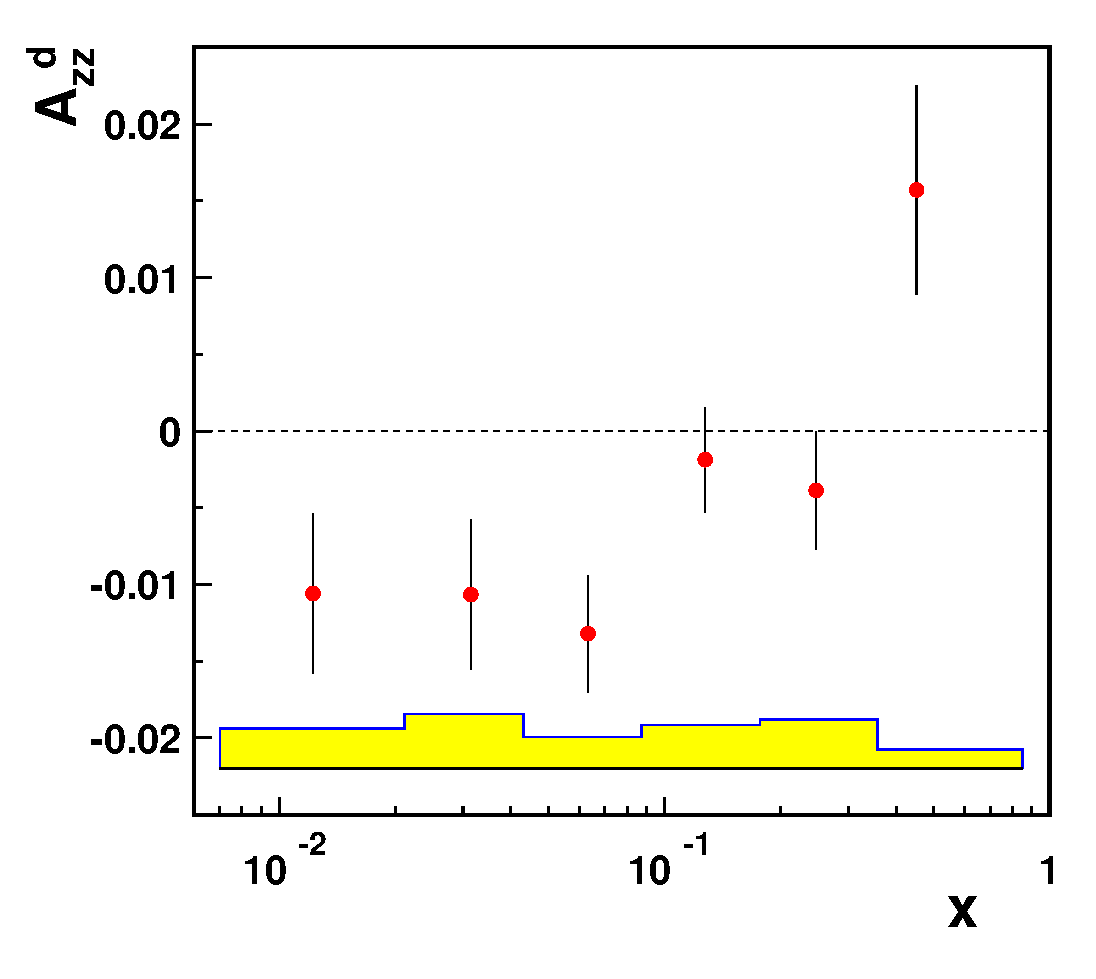
\includegraphics[angle=0,width=4.in]{figs/azzfinal.eps}
%\caption{\label{HERMES_AZZ} HERMES measurement of the inclusive tensor asymmetry A$_{zz}$ of the deuteron.
%The error band displays the total systematic uncertainty.
%{\it Reproduced from~\cite{Riedl:2005jq}.}}
%\end{center}\end{figure}

%\begin{figure}
%\begin{center}
%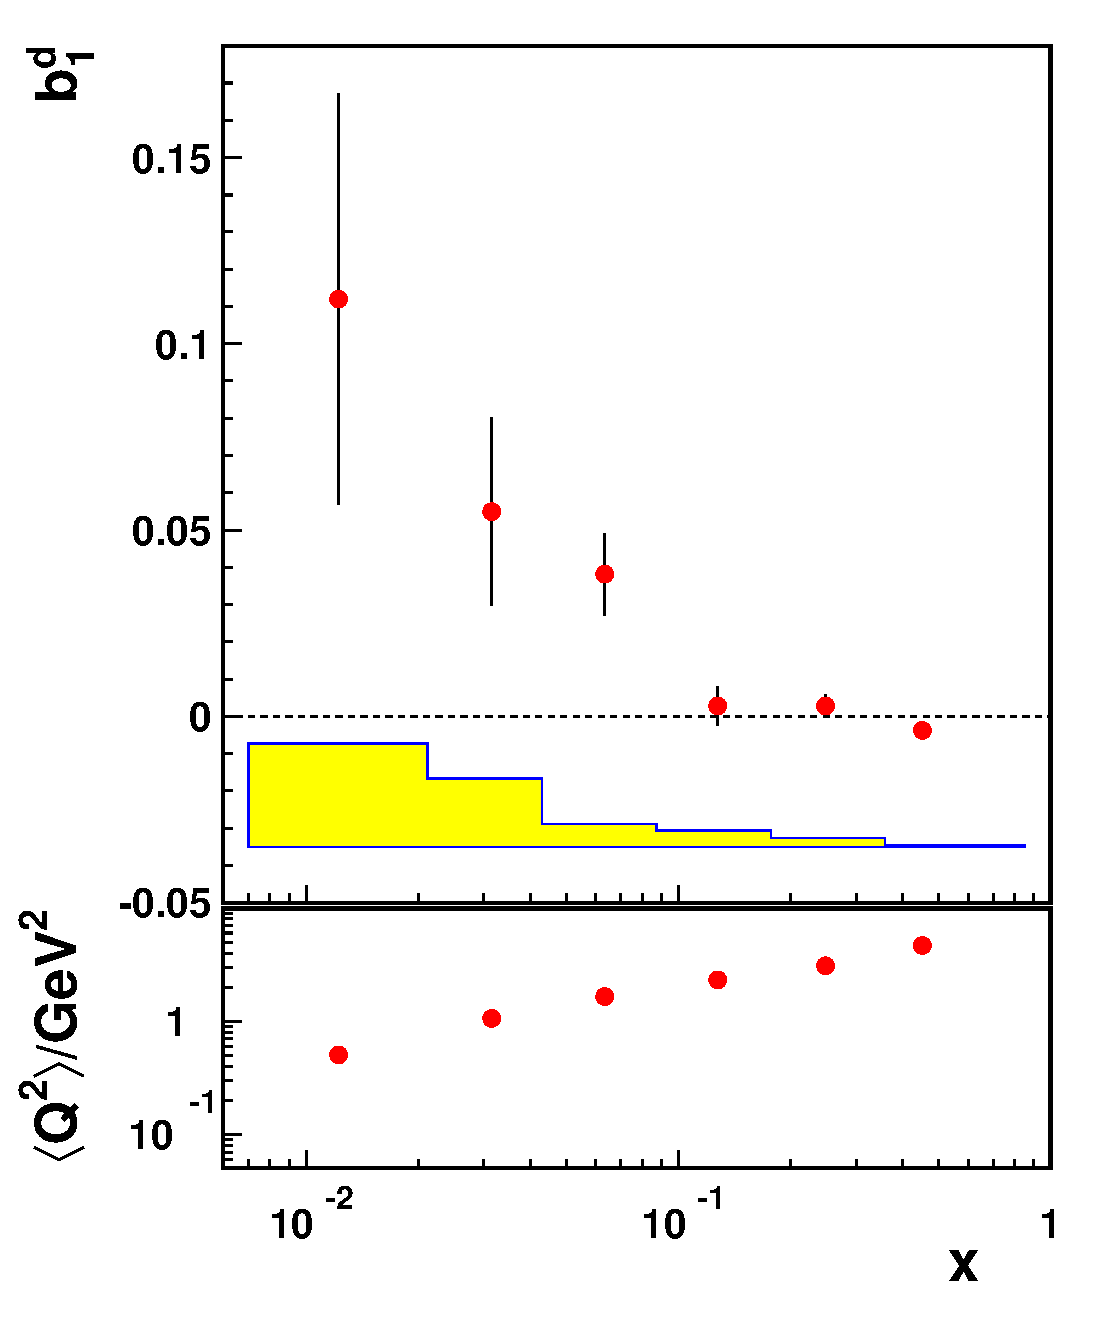
\includegraphics[angle=0,width=4.1in]{figs/b1final.eps}
%\caption{\label{HERMES_B1D} HERMES measurement of the inclusive tensor structure function b$_1^d$ and the average $Q^2$ for each x-bin.  The error band displays the total systematic uncertainty.
%{\it Reproduced from~\cite{Riedl:2005jq}.}}
%\end{center}\end{figure}


\begin{figure}
\begin{center}
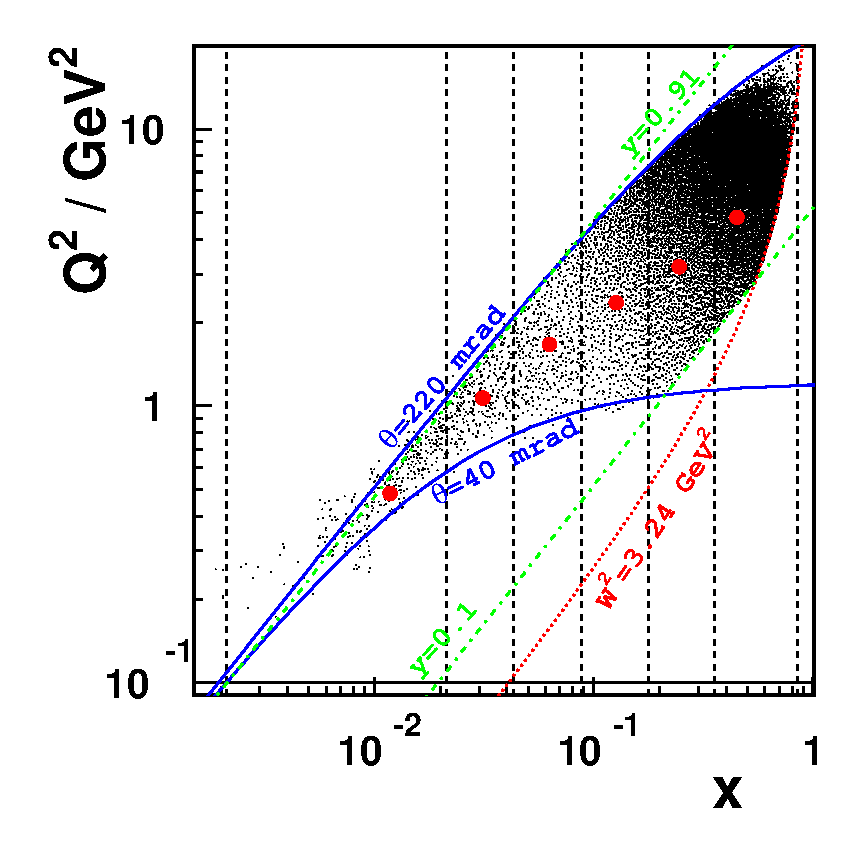
\includegraphics[angle=0,width=0.45\textwidth]{figs/kineplane.eps}
\caption{\label{HERMES_KIN} Kinematic coverage of the HERMES measurement.  The dashed vertical lines indicate the borders
of the bins in x, the dots their centers of gravity. The solid curves
indicate the
vertical acceptance of the spectrometer, defined by its aperture.
In addition, the
kinematic cuts imposed on the variables Q$^2$, y
and W$^2$ are shown. 
%The W$^2$ cut suppresses the nuclear resonance region.
{\it Reproduced from~\cite{Riedl:2005jq}.}}
\end{center}\end{figure}


The HERMES collaboration  made the first measurement~\cite{Riedl:2005jq,Airapetian:2005cb} of
$b_1$ in 2005.
The experiment explored the low $x$ region of $0.001<x<0.45$ for  $0.5<Q^2<5$ GeV$^2$.  
An atomic beam source was used to generate a deuterium gas target with high tensor polarization.  
The HERA storage ring provided 27.6 GeV positrons incident on the internal gas target.

As displayed in Fig.~\ref{HERMES_AZZ}, the tensor asymmetry A$_{zz}$  was found to be 
non-zero at about the  two sigma level, with an apparent zero crossing around $x=0.3$. %  for $x < 0.1$.  
%
The tensor structure function $b_1$ exhibits a steep rise as $x\to 0$, which is qualitatively
in agreement with the predictions of coherent double-scattering models. See for example Ref.~\cite{Edelmann:1997ik}.  The authors of Ref.~\cite{Airapetian:2005cb} interpret the rapid rise at low $x$ in terms of the same mechanism that leads to nuclear shadowing in unpolarized scattering, i.e. double scattering of the lepton, first from the proton, then from the neutron, with sensitivity to the spatial alignment of the two nucleons.
%The Close-Kumano integral (Eq.~\ref{cksum}) was evaluated and found to be:
%\begin{eqnarray}
%\int_{0.0002}^{0.85} b_1(x) dx = 0.0105 \pm 0.0034 \pm 0.0035
%\end{eqnarray}
%which result possibly indicates a breaking of the Close-Kumano sum rule, and consequently a 
%tensor-polarized quark sea.
%%
%%

As is often the case with a pioneer measurement, the precision of the results leaves some
room for ambiguity.  Despite the surprisingly large magnitude and interesting trend of the data, 
all points are roughly within two sigma from zero, which calls for a higher precision measurement.
Another issue is that some of the HERMES momentum transfer values are low 
(see Fig.~\ref{HERMES_KIN}), so that quark structure functions may not be the correct language. 
The $Q^2$ variation in each $x$-bin is also quite wide ($\approx$10 GeV$^2$ for $x\sim 0.3$), which complicates
the interpretation of this data, since  several models predict significant $Q^2$-dependence of
 $b_1$. See for example Fig.~\ref{xb1_pred}.


%\begin{figure}\begin{center}
%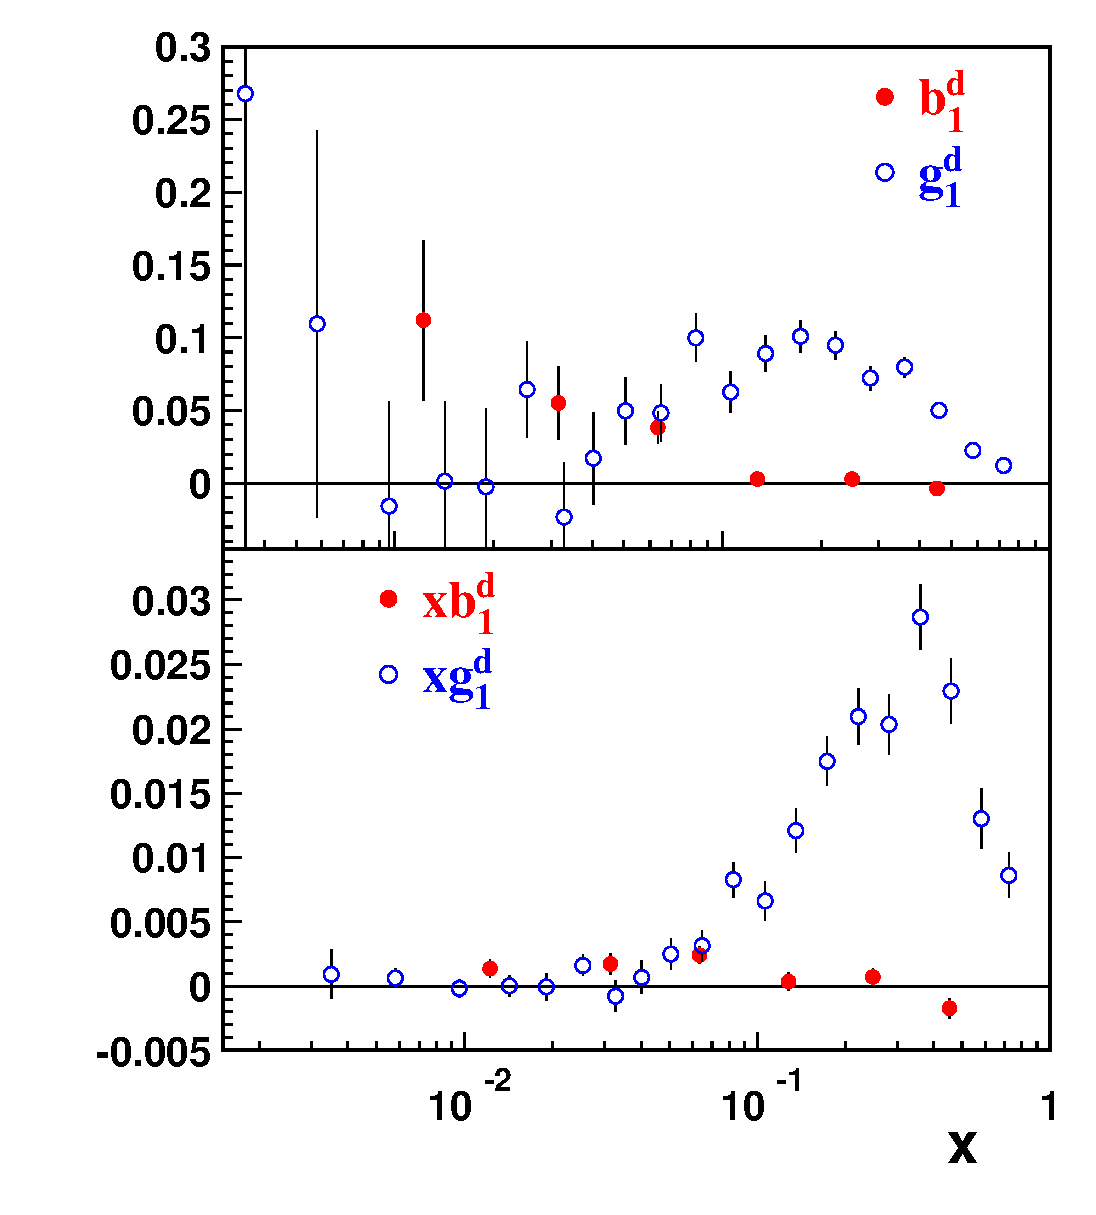
\includegraphics[angle=0,width=3.1in]{figs/b1g1.eps}
%\caption{\label{}\footnotesize
%{\it Reproduced from~\cite{Riedl:2005jq}.}}
%\end{center}\end{figure}

%\begin{figure}\begin{center}
%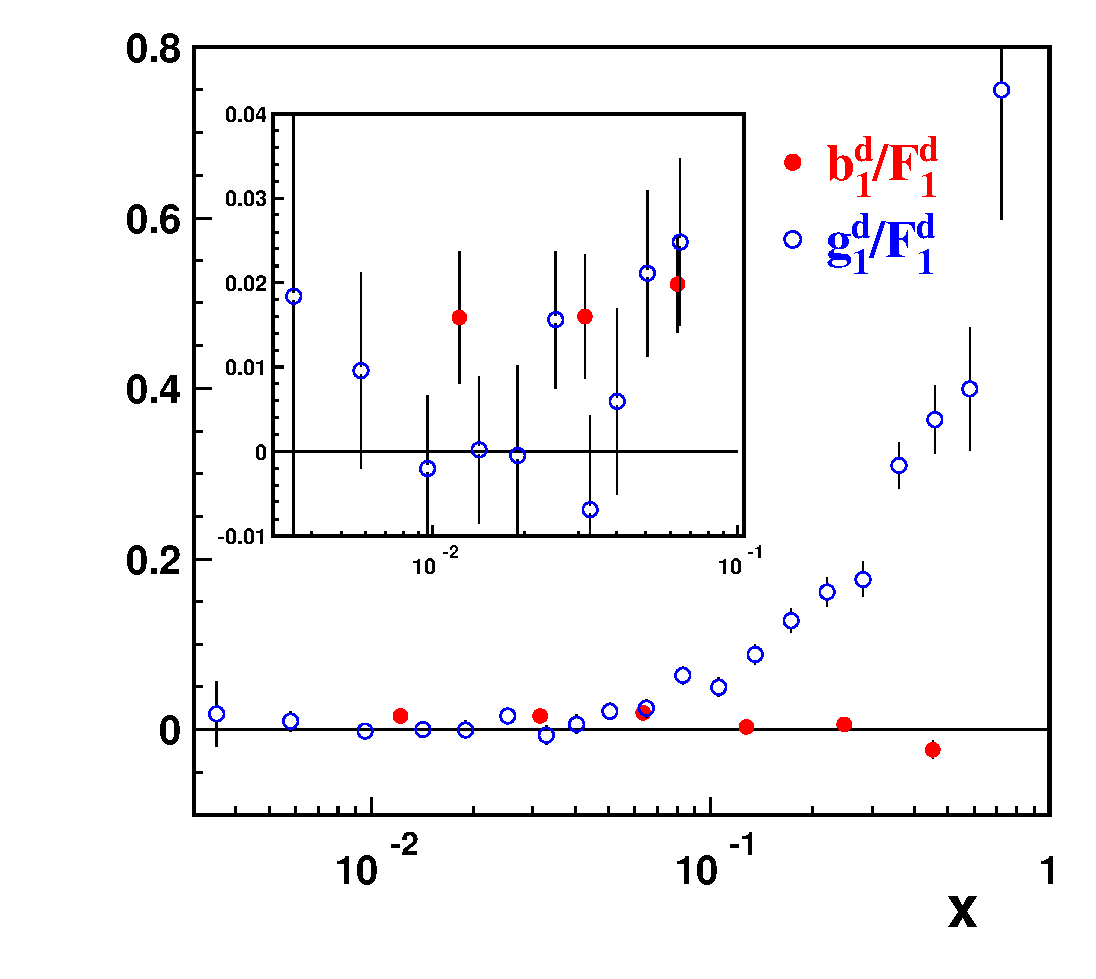
\includegraphics[angle=0,width=3.1in]{figs/b1g1overf1.eps}
%caption{\label{}\footnotesize
%{\it Reproduced from~\cite{Riedl:2005jq}.}}
%\end{center}\end{figure}

%\begin{figure}\begin{center}
%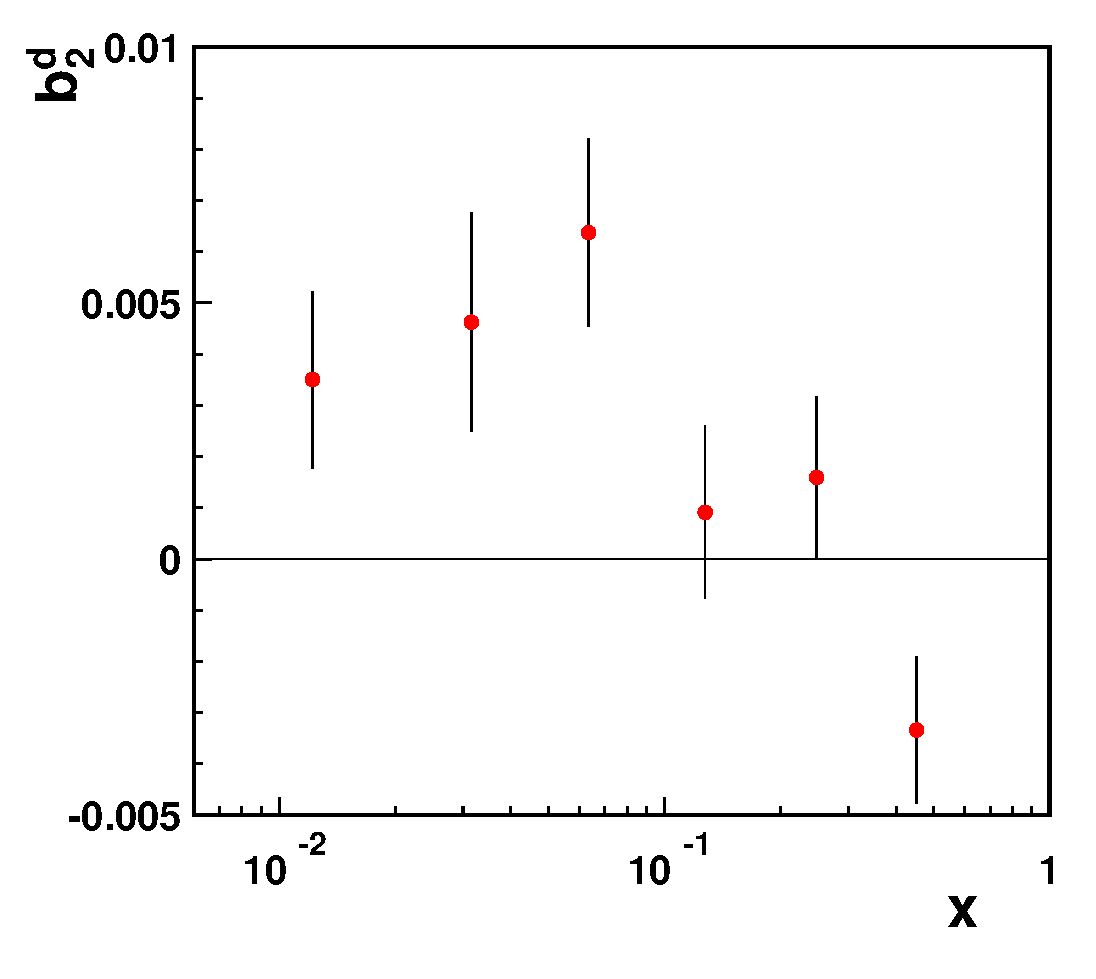
\includegraphics[angle=0,width=3.1in]{figs/b2theo.eps}
%\caption{\label{}\footnotesize
%{\it Reproduced from~\cite{Riedl:2005jq}.}}
%\end{center}\end{figure}

